\documentclass[__main__.tex]{subfiles}

\begin{document}

\qtitle{О}{04}
Найти угловое распределение дифракционных минимумов при дифракции на решетке, период которой равен $d$, а ширина щели равна $b$.\\ 

Дифракционная решетка представляет собой простой спектральный прибор, т.е. прибор, позволяющий исследовать спектральный состав света. Она позволяет различать компоненты, которые для глаза кажутся одного цвета.
Дифракция Фраунгофера – дифракция в параллельных лучах, и поэтому она обладает важным свойством: дифракционные картины от двух смещенных друг относительно друга объектов накладываются друг на друга без смещения. Именно это свойство используется в дифракционной решетке, представляющей собой большое количество $N$ одинаковых щелей, расстояние между которыми постоянно. Расстояние  $d$  между серединами соседних щелей называется периодом решетки. Ширину щели, как и раньше, будем обозначать буквой $b$.

\begin{figure}[h]
	\begin{center}
		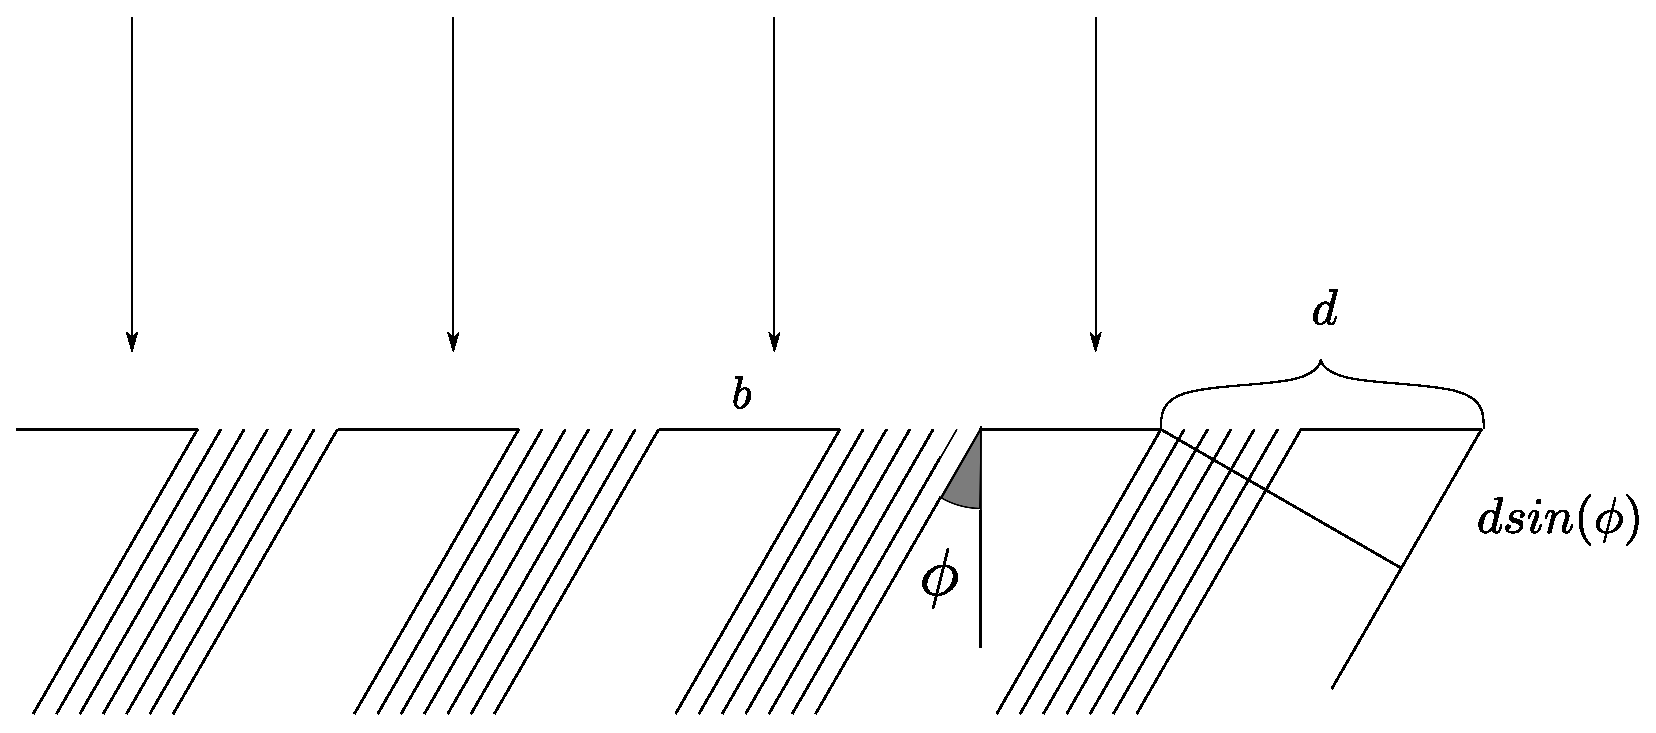
\includegraphics[width=0.5\linewidth]{img/o-07_1.eps}
		\caption{Дифракционная решетка}
	\end{center}
\end{figure}

Пусть $E^{(1)} (\varphi)$ - световое поле, посылаемое одной щелью под углом $\phi$ к нормали. Тогда поле от $N$ записывается как суперпозиция:
$$E^{(N)}(\varphi) = E^{(1)}(\varphi)(1 + e^{ik\Delta} + ... + e^{ik(N-1)\Delta}),$$
где $\Delta = d\sin \varphi$ - оптическая разность хода между лучами, идущими от соседних щелей. Слагаемые в скобке образуют геометрическую прогрессию с суммой:
$$\frac{1-e^{iNk\Delta}}{1-e^{ik\Delta}} = \frac{e^{iNk\frac{\Delta}{2}}}{e^{ik\frac{\Delta}{2}}}\cdot \frac{e^{iNk\frac{\Delta}{2}} - e^{-iNk\frac{\Delta}{2}}}{e^{ik\frac{\Delta}{2}} - e^{-ik\frac{\Delta}{2}}},$$
Введем для удобства переменную $\delta = \frac{kd\sin\varphi}{2}$, получаем:
$$E^{(N)}(\varphi) = E^{(1)}(\varphi)\frac{e^{iN\delta}}{e^{i\delta}}\cdot \frac{\sin N\delta}{\sin\delta}$$
Для интенсивности:
$$I^{(N)}(\varphi) = I^{(1)}(\varphi)\frac{\sin^2 N\delta}{\sin^2\delta}$$
Если $\sin \delta$ в знаменателе дает 0, то и числитель равен 0. это случается, когда $\delta = m\pi \rightarrow kd\sin\varphi = 2m\pi$. Получаем условие для главного максимума:
$$d\sin(\varphi^{max}_m) = m\lambda,$$
где $m = 0, \pm 1, \pm 2...$ - порядок главного максимума. Интенсивность в главном максимуме очень велика. Поскольку синус меньше единицы, число наблюдаемых главных максимумов удовлетворяет условию:
$$m < \frac{d}{\lambda}$$
Числитель дроби в формуле для интенсивности также может обращаться в 0 при $N\delta = p'\pi, $ но $\delta \neq m\pi$, $p' = \pm 1, p\pm 2, ...$, т.е. когда $d\sin(\varphi ^{min}_{p'}) = \frac{p'}{N}\lambda, \frac{p'}{N} \neq m$  
Это минимумы с нулевой интенсивностью, условия можно записать в более удобном виде. Если $p' = 0, $ то $m = 0$ и это максимум нулевого порядка. Далее годятся все $p' = \pm1, \pm2, ... , \pm(N-1). $ При $p' = \pm N$ получаются симметричные главные максимумы первого порядка. Далее отношение $\frac{p'}{N}$ можно записать как $1 + \frac{p}{N}, p =  \pm1, \pm2, ... , \pm(N-1)$. Далее появляются максимумы второго порядка. Продолжая это рассмотрение, приходим к условию минимумов:
$$d \sin(\varphi^{min}_{m, p}) = (m + \frac{p}{N})\lambda$$
Мы видим, что между ближайшими друг к другу максимумами находится $N - 1$ минимумов. Ясно, что минимумы отделены друг от друга максимумами, и если это не главные максимумы, то они называются второстепенными или побочными. В частности, для ближайших к $m$-му главному максимуму минимумов:
$$d\sin(\varphi^{min}_{m, \pm1}) = (m \pm \frac{1}{N})\lambda$$

Из всего вышесказанного можно сделать вывод, что угловое распределение минимумов будет иметь следующий вид:

\begin{gather*}
	Nd\sin\varphi = n\lambda\\
	d\sin\varphi \neq k\lambda\\
	b\sin\varphi = c \lambda,
\end{gather*}

где $n, k, c$ - некоторые целые числа.
\end{document} 
